\documentclass[twoside,10pt]{report}
\usepackage{/Users/bradenhoagland/latex/styles/toggles}
\toggletrue{sectionbreaks}
%\toggletrue{sectionheaders}
\newcommand{\docTitle}{Algebraic Topology}
\usepackage{/Users/bradenhoagland/latex/styles/common}
\importStyles{modern}{rainbow}{boxy}

%\renewcommand{\theenumi}{\alph{enumi}}

\begin{document}
\tableofcontents

%--------------------------------------------------------------------------------
% CW Complexes
%--------------------------------------------------------------------------------
\section{CW Complexes}

For $n \geq 1$, an \textbf{$n$-cell} (or a cell of dimension $n$) is a space homeomorphic to the open ball $B^{n}$. A 0-cell is said to just be a point.

\warn{Figure for 0, 1, 2-cells.}

\warn{Figure for simple CW complex.}

A CW complex $X$ is then built inductively by gluing cells of different dimension together. We can represent this gluing via continuous maps $D^{n}\to X$:
\begin{itemize}
	\item $\p D^{n}\to X$ says how the cell is glued to existing lower-dimensional cells in $X$;
	\item $B^{n}\to X$ says where the new stuff goes.
\end{itemize}
Thus we only really need to specify $\p D^{n}\to X$. Since $\p D^{n} \cong S^{n-1}$, this is the same as specifying a map $S^{n-1}\to X$. Formally, gluing $D^{n}$ to $X$ via a map $\varphi:D^{n}\to X$ is represented with the space
\[
	\frac{X \sqcup D^{n}}{x \sim \varphi(x)}.
\] But this notation is messy, so we'll use the notation $X \cup_{\varphi}D^{n}$ instead.

\begin{figure}[H]
	\centering
	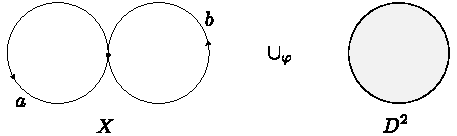
\includegraphics[scale=1]{fig/glue-not-htpy-equiv.pdf}
	%\caption{}
\end{figure}

The map $\varphi$ is important, as two different gluing maps can yield spaces that aren't even homotopy equivalent. For example, if we glue $D^{2}$ to $X$ above via the constant map $x \mapsto \bullet$ (the intersection point of $X$), then we get $S^{1}\vee S^{1}\vee S^{2}$, which has $\pi_1 = \mathbb{Z} * \mathbb{Z}$. If we instead map $\p D^2$ to $aba^{-1}b^{-1}$, then we get the torus, which has fundamental group $\mathbb{Z}^2 \not\cong \mathbb{Z}*\mathbb{Z}$.

In general, cell structures on a topological space are not unique. For example, the circle can be represented with $n$ 0-cells and $n$ 1-cells for any $n \geq 1$.
\begin{figure}[H]
	\centering
	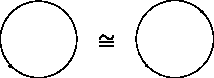
\includegraphics[scale=1.4]{fig/cell-not-unique.pdf}
\end{figure}

\begin{defn}[]
A \textbf{CW complex} $X$ is a collection of disjoint cells $e_{\alpha} \subset X$ such that
\begin{enumerate}
	\item $X$ is Hausdorff;
	\item $\bigcup_{\alpha}e_{\alpha}=X$;
	\item Closure finiteness: for each $e_{\alpha}$ with dimension $\geq 1$, there is a continuous map $\varphi_{\alpha}:D^{n}\to X$ such that
		\begin{itemize}
			\item $B^{n} \cong e_{\alpha}$ via $\varphi_{\alpha}$;
			\item $\varphi_{\alpha}$ maps $\p D^{n}$ to a finite union of cells, each of dimension $\leq n-1$.
		\end{itemize}
	\item Weak topology: $A \subseteq X$ is closed $\iff A \isct \overline{e}_{\alpha}$ is closed in $\overline{e}_{\alpha}$ for all $\alpha$. Here, $\overline{e}_{\alpha}=\varphi_{\alpha}(D^{n})$. \warn{is this closure of $e_{\alpha}$?}
\end{enumerate}
\end{defn}

\begin{note}[]
Each $\varphi$ is a map $D^{n}\to X$, but the cell being added is only the image of $B^{n}$. The image of $\p D^{n}$ is the union of lower-dimensional cells that the new cell is being glued to.
\end{note}

A CW complex is \textbf{finite} if it has finitely many $e_{\alpha}$, and it is \textbf{$n$-dimensional} if the max dimension of all its cells is $n$.

We can build CW complexes inductively, starting with 0-cells and adding in higher dimensional cells to fill in the gaps.

\begin{defn}[]
The \textbf{$m$-skeleton} of a CW complex $X$ is
\[
X_{m} \doteq \bigcup_{}\left\{ e_{\alpha}\;|\; \dim e_{\alpha}\leq m \right\}.
\] 
\end{defn}

Thus when $X$ is $n$-dimensional, $X_{n}=X$. To build $X$, we start with its 0-skeleton and then glue on its higher dimensional cells to get its higher dimensional skeletons, eventually recovering $X$ itself. If $e_{\alpha}^{n}$ denotes $e_{\alpha}$ being an $n$-cell, then
\begin{align*}
	X_{n} &= X_{n-1} \;\cup\; (\cup_{\alpha} e_{\alpha}^{n}) \\
	      &= X_{n-1} \;\cup_{\varphi_{\alpha}}\; \left( \cup_{\alpha}D^{n} \right)
\end{align*}
since $\varphi_{\alpha}(\p D^{n})$ is contained in $X_{n-1}$.

\begin{ex}
	The torus is 2-dimensional since its 2-skeleton is just itself.
	\begin{itemize}
		\item 0-skeleton: $\bullet$.
		\item 1-skeleton: $S^{1}\vee S^{1}$.
		\item 2-skeleton: $T^2$.
	\end{itemize}
\end{ex}


%+-------------------+
%| +---------------+ |
%| |    Chapter    | |
%| +---------------+ |
%+-------------------+
% The Fundamental Group

\chapter{The Fundamental Group}

%--------------------------------------------------------------------------------
% The Fundamental Group
%--------------------------------------------------------------------------------
\section{The Fundamental Group}

\warn{Add in notes from last year?}

\begin{prop}
	All paths (regardless of endpoints) are homotopic in a path-connected space.
\end{prop}
\begin{proof}
	All paths are clearly homotopic to both of their endpoints. Thus we can shrink down one path to an endpoint, follow a path to one of the other path's endpoints, then expand out.
\end{proof}

\begin{note}[]
If two paths with the same endpoints are homotopic, assume they're homotopic rel the endpoints, i.e. path homotopic.
\end{note}

\begin{prop}
	Homotopy rel $A$ is an equivalence relation.
\end{prop}

Path multiplication is just concatenation (with normalization to ensure that everything happens on $I$ still). Although paths are maps, we write path multiplication left to right in the algebraic style.

This is \textit{not} a group operation on paths because of the time normalization; however, $[fg] \doteq [f][g]$ \textit{is} a group operation on homotopy classes. It's also well defined in the first place since if $f \simeq f'$ and $g \simeq g'$ as paths, then $fg \simeq f'g'$.

\begin{defn}[]
	The \textbf{fundamental group} of $X$ at $x_0$ is the homotopy classes of loops at $x_0$ with the group operation $[fg]\doteq [f][g]$.
\end{defn}

\begin{prop}
	In the same path component, all fundamental groups are iso via the \textbf{change of basepoint iso}: if $h$ is a path from $x$ to $y$, then
	\begin{align*}
		\pi_1(X,x_1) &\stackrel{\sim}{\to } \pi_1(X,x_0) \\
		[f] &\mapsto [h f \overline{h}].
	\end{align*}
\end{prop}
\begin{proof}
	The change of basepoint map is a homomorphism with inverse $[f] \mapsto [\overline{h}fh]$.
\end{proof}

$\pi_1$ is a covariant functor $\cat{Top}_{*}\to \cat{Grp}$.
\begin{itemize}
	\item A map $\phi:X\to Y$ induces a homomorphism $\phi_{*} : [f] \mapsto [\phi f]$.
	\item The induced maps are covariant: $(\phi\psi)_{*} = \phi_{*}\psi_{*}$.
	\item Identities are preserved: $(1_{X})_{*} = 1_{\pi_1(X)}$.
\end{itemize}

\begin{prop}
If $f,g:X\to Y$ are homotopic, then $f_{*} = g_{*}$.
\end{prop}

\begin{prop}
	If $X \cong Y$, then $\pi_1(X)\cong \pi_1(Y)$.
\end{prop}
\begin{proof}
	Functors preserve isos.
\end{proof}

%--------------------------------------------------------------------------------
% Homotopy Equivalence
%--------------------------------------------------------------------------------
\section{Homotopy Equivalence}

\begin{defn}[]
We say $X$ and $Y$ are \textbf{homotopy equivalent}, written $X \simeq Y$, if there exist
\[
	\begin{tikzcd}
		X \rar[bend left]{f} & Y \lar[bend left]{g}
	\end{tikzcd}
\] such that $gf \simeq 1_{X}$ and $fg \simeq 1_{Y}$.
\end{defn}

As it turns out, this is all we need to have isomorphic fundamental groups.

\begin{thrm}[]
	If $f,g:X\to Y$ are homotopic, then
	\[
	\begin{tikzcd}
		\pi_1(X,x_0) \rar{f_{*}} \arrow[dr, "g_{*}"'] & \pi_1(Y,f(x_0)) \dar[dashed]{\sim} \\
		& \pi_1(Y,g(x_0))
	\end{tikzcd}
	\] 
\end{thrm}
\begin{proof}
	Suppose $f \simeq g$ via $F$, then $h(t) \doteq F(x_0,t)$ is a path from $f(x_0)$ to $g(x_0)$. We then use this $h$ in the change of basis iso. \warn{Show it commutes.}
\end{proof}

\begin{cor}
	\label{htpy-equiv-iso-fundamental-grp}
	If $X \simeq Y$ via $f:X\to Y$, then $\pi_1(X,x_0) \cong \pi_1(Y,f(x_0))$ via $f_{*}$.
\end{cor}

\begin{defn}[]
A space is \textbf{contractible} if it's homotopy equivalent to a point. This is the same thing as requiring the identity map to be \textbf{nullhomotopic}, i.e. homotopic to a point.
\end{defn}

%--------------------------------------------------------------------------------
% Deformation Retracts
%--------------------------------------------------------------------------------
\section{Deformation Retracts}

\begin{defn}[]
	Suppose $A \subseteq X$, then $r:X\to A$ is a \textbf{retraction} onto $A$ if $ri=1_{A}$, i.e. it fixes $A$.
\end{defn}

\begin{defn}[]
	A \textbf{deformation retract} of $X$ onto $A$ is a homotopy $F:X\times I\to X$ such that
	\begin{align*}
		F_0 &= 1_{X}, \\
		F_1(x) &\in A, \\
		F_{t}|_A &= 1_{A}.
	\end{align*}
	A \textbf{weak deformation retract} is the same, exact $F_t$ need only map $A$ into itself.
\end{defn}

Note that a deformation retract is a homotopy between the identity on $X$ and a retraction $F_1$ of $X$ onto $A$.

\begin{prop}
If $A$ is a deformation retract of $X$, then $A \simeq X$ via the inclusion $A \inj X$.
\end{prop}
\begin{proof}
	By definition, $F_1 \circ i = 1_{A}$. Also, $i \circ F_1 \simeq 1_{X}$ via $F$.
\end{proof}

\begin{cor}
	If $A$ is a deformation retract of $X$, then $\pi_1(A,a_0) \cong \pi_1(X,a_0)$.
\end{cor}
\begin{proof}
	Apply \Cref{htpy-equiv-iso-fundamental-grp} with the homotopy equivalence $A \inj X$.
\end{proof}

\warn{still homo equiv if weak DR. See HW.}

\warn{How much will we use weak DR's?}


\end{document}
